\chapter{Approach}
\label{cha:approach}
In this chapter, we will discuss in detail, the process of applying the Kernel PCA on different text data-sets and how to obtain the word embeddings using these KPCA embeddings in the skip gram model. Using this approach, we can thus make use of morphological similarities to learn semantic and syntactic similarities between the words. We will be using our approach to generate word embeddings for both morphological language, German as well as non-morphological language, English. There are many datasets available at our disposal for exploring various text analysis problems in both of these languages. We will be mainly working with \texttt{text8}, \text{wikidump2016} and \texttt{20News group} datasets for English and \texttt{news.2013.de} for German.

\section{Kernel Principal Component Analysis on Strings}\label{secKPCA}
Kernel Principal Component Analysis is a powerful algorithm in the field of machine learning. When applied, it helps in solving non-linear clustering problems in a higher dimensional space. In the following section, we will be discussing about applying Kernel PCA on "text data". As discussed in earlier chapters, when we delve into the text mining, we need word vectors to be represented in a vector space. It is very intuitive to say that since the vocabulary is quite large, we need the representation of words to be in a higher dimensional space so that we can easily represent words and the relationship them. Hence making clustering problem solvable. Kernel PCA is very helpful as it enables us to achieve this goal without explicitly working in a high dimensional space.\\
Since our goal is to cluster morphological similar words together, in the first step, we start with computing the \texttt{String similarity} between words. This similarity is computed by a function which takes the number of common \textit{n}-grams between two strings in the given vocabulary, $\mathbf{V}$. We also know that if two words have lot of \textit{n}-grams in common, then there is a high probability that these words will lie close to each other in the feature space. One such example of the similarity function is represented in the equation, \ref{eq1.1}.
 \begin{equation}\label{eq1.1}
 \mathcal{S}(s_1,s_2) = \frac{2\times\mid B_1\cap B_2\mid}{\mid B_1 \mid + \mid B_2 \mid}
 \end{equation}
 In the above equation, \ref{eq1.1}, $\mathcal{S}$ represents the similarity function computed between the words, $s_1$ and $s_2$. $B_1$ and $B_2$ are the set of \textit{n}-gram of these words. Given the vocabulary, $\mathbf{V}$, we can compute this similarity function of every word in $\mathbf{V}$ and thus obtain a similarity matrix, $\mathbf{S}$ of shape $V\times V$.
 The next step is to cluster the similar words together. Here kernel PCA comes into play. We kernelize the similarity matrix using the non-linear kernel function, $\mathcal{K}$, which generates a Kernel matrix $\mathbf{K}$ of shape $V\times V$.\\
  For applying this algorithm, choosing an appropriate kernel function is very important since this function will determine the dimension and hyperplane where clustering can be achieved. There are many kernel functions available such as Logistic kernel,  Epanechnikov kernel, Cosine kernel, Gaussian kernel and Polynomial kernel of degree, p. Clustering of words works best in languages like \textit{German} and \textit{Turkish} since the words with similar meaning have same morphemes. Because of the fact that the Gaussian kernel function works in an infinite dimensional space, it becomes a very common choice for solving such problems. Clustering using Gaussian kernel PCA is demonstrated in figures \ref{fig:kgaussianen} and \ref{fig:kgaussiande}.\\
  \begin{figure}[H]
  	\centering
  	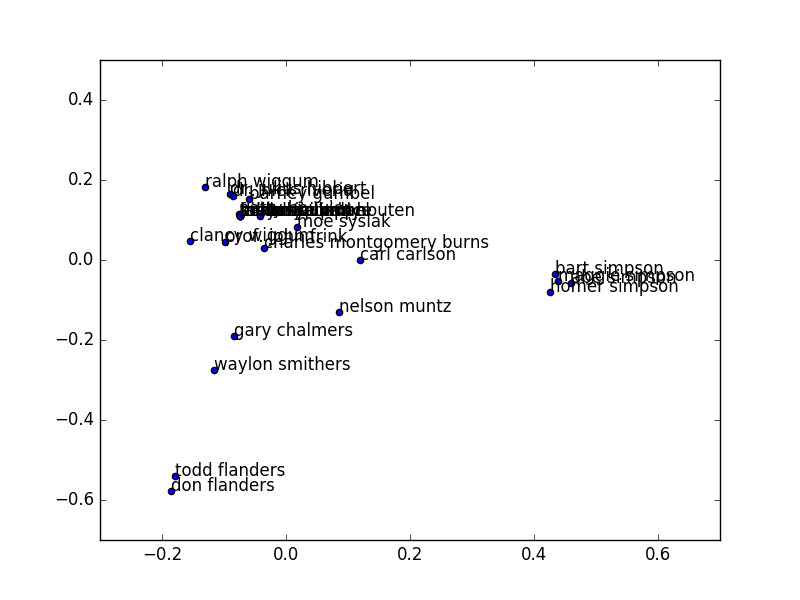
\includegraphics[width=15cm,height=12cm,keepaspectratio]{files/KERNELPCA/gaussianN3en.png}
  	\caption{Kernelized PCA using Gaussian kernel on English words using \textit{n}-grams similarity where \textit{n}=3}
  	\label{fig:kgaussianen}
  \end{figure}
   The resulting kernel matrix can be seen as vectors in a very high dimensional space. To visualize these vectors in lower dimensional space, we need to select $d$ eigenvectors of this Kernel matrix, $\mathbf{K}$. By selecting $d$ eigenvectors($\mathbf{v_d}$) corresponding to the \textit{first} $d$ eigenvalues($w_d$), we can generate a matrix $\mathbf{P}$, known as the "Projection Matrix". We should also note that selecting eigenvectors corresponding to the first $d$ eigenvalues is important because this makes sure that we have maximum variance and thus do not loose any vital information.
   \begin{equation}
   \mathbf{P} = \big[\frac{\mathbf{v_1}}{w_1},...,\frac{\mathbf{v_d}}{w_d}\big]
   \end{equation}
   The KPCA embeddings, $\mathbf{e}$ of each word in the given vocabulary, $V$ can be computed by projecting the kernel matrix row of the corresponding word on the projection matrix.
   \begin{equation}
    \mathbf{e}= \mathbf{P}^T \mathbf{k}
   \end{equation}
   where: 
   \begin{enumerate}
   	\item $\mathbf{e}$ is each row in the vector embeddings, $\mathbf{W}$.
   	\item $\mathbf{k}$ is the row of kernel matrix $\mathbf{K}$.
   \end{enumerate}
   
  \begin{figure}[H]
 	\centering
 	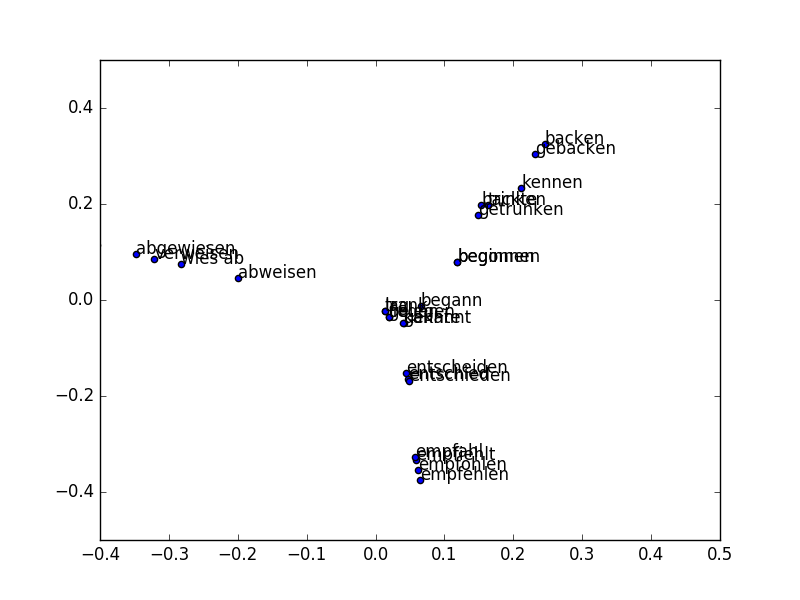
\includegraphics[width=15cm,height=12cm,keepaspectratio]{files/KERNELPCA/gaussianN3de.png}
 	\caption{Kernelized PCA using Gaussian kernel on German words using \textit{n}-grams similarity where \textit{n}=3}
 	\label{fig:kgaussiande}
 \end{figure}
Thus we can generate the "KPCA embeddings of dimension $\mathit{d}$" of a set of words. The beauty of this method is that it can be applied to any kind of non-numeric data. 
\section{Word vectors using Kernel PCA and Skip-Gram model}
 In this section, we will explore the idea of improving the word2vec skip-gram model by using word embeddings generated from Kernel PCA (KPCA embeddings). We propose an extension to the skip-gram model by feeding the model with these embeddings. The main motivation behind the approach is to use the \textit{root/morpheme} information encoded in the structure of the word, which is not considered by the word2vec models. Similar to the skip-gram model, our model also follows, an unsupervised approach for learning word embeddings. The key difference is that we are feeding the network, explicitly with the morphological similarities learned using KPCA. Hence we can say that our model uses the semantic, syntactic and morphological information in the words and the text to generate better word vectors.
 \subsection{Pre-processing the dataset}
 We are using different data-sets like Text8, 20 Newsgroups dataset, enWiki2016 dump, news.2013.de.shuffled.corpus for generating and for evaluating KPCA word embeddings. Every dataset is a collection of web articles crawled from news websites or Wikipedia. These raw text corpuses have a large amount of irrelevant text which we do not want our network to learn. Such text includes capitalization, punctuation, foreign text, tables, markup, formatting, hypertext links, and XML structure such as timestamps, authorship, and comments. This preprocessing step help us to clean the text by removing all the convert to lowercase letters and spaces, spell digits. Thus we need to filter out the junk and generate readable English.\\
 Text8 corpus is a cleaned Wikipedia text and can be used directly but we need to clean the other datasets. Text8 corpus is generated using the preprocessing script by \textit{Matt Mahoney} \footnote{\url{http://cs.fit.edu/~mmahoney/compression/text.html/}}.The script removes any text that would not be visible on the Wikipedia website besides removing the punctuations. When the text is reduced to only letters, digits, and nonconsecutive spaces, the resulting text is about 70\% of the original size. This is expanded to 74\% after spelling out digits (a common technique in speech models).\\ 
 For German text corpus, we need to perform some additional preprocessing steps. German words consist of umlauts which need to be transformed. 
 \begin{center}
 	 For example: {\"a} -> ae and \ss -> ss.
 \end{center}
 At the end, the data has to be stored in a text file or to be supplied in a continuous stream with each sentence per line with each line, being UTF-8 encoded strings/tokens separated by spaces. This file can now be used to construct a vocabulary and to train any model for text mining problems.
 \subsection{Implementing Kernel PCA on words in a vocabulary}\label{sub:vw}
 After cleaning the text corpus, we need to generate the vocabulary from this dataset. The major challenge is how to deal with a huge vocabulary. For applying Kernel PCA, we need to find the eigenvalues and eigenvectors of the Kernel matrix which is used to generate Kernel PCA embeddings. Since this computation is quite expensive and has to be done on the whole vocabulary so it is better to select an optimal subset of vocabulary to generate \textbf{Projection matrix} which can then be used to generate KPCA word embeddings for out-of-vocabulary words. The vocabulary is generated from most frequently used in the text corpus. Therefore the vocabulary consists of most frequently occurring, $\mathbf{V}$, words. In this work, we have also tried to evaluate the performance of the model with different vocabulary sizes.\\ 
 %As per \footnote{http://www.cs.trincoll.edu/~crypto/resources/LetFreq.html}, the %average length of English words is 4.5 letters, so we created a vocabulary of %words of length between 4 and 8. This created a vocabulary of size, represented %by $\mathbf{V'}$.
\begin{center}
Here $\mathbf{V}$ sizes used are 20,000 words, 30,000 words, 118,000 words.
\end{center}
 Following the steps mentioned in \ref{secKPCA} to compute the Projection matrix and Kernel PCA embeddings of dimension, $d$ for the words in the vocabulary.
 
 \subsection{Implementing Kernel PCA on out-of-vocabulary words}\label{oov}
 This step is quite straightforward to implement once we have the projection matrix of the vocabulary words. The projection matrix can be used to generate the KPCA vectors for the words which are not present in the vocabulary. By using this step, we can increase our vocabulary size for training data-sets with large vocabulary or get KPCA vectors for out of vocabulary words.\\
 
 For any word $s_n$, which is not in the vocabulary $\mathbf{V}$, we need to compute the kernel vector of dimension $\mathbf{d}$, with respect to all the words in the vocabulary. To compute the KPCA vector of $s_n$, we then project its kernel vector on the projection matrix, demonstrated in equation \ref{eq:4.4}:
 \begin{equation}\label{eq:4.4}
 	\mathbf{e}_n =\mathbf{P}^T \mathbf{k}_n
 \end{equation} 
 where:
 \begin{equation}
	 \mathbf{k}_n = \mathcal{K}(\mathcal{S}(s_n,\mathbf{V}))
 \end{equation}
This also helps in overcoming the disadvantage of word2vec model which excludes all the words with low-frequency count or may not be present in the dataset. At this stage, we can compute KPCA word embeddings for any of the Out-of-Vocabulary words. We should also note that these KPCA word vectors are only morphologically similar. We need to train them using a skip gram model to include semantic and syntactic similarities.

\subsection{Implementing word2vec model(Skip gram) with KPCA Embeddings in Tensor flow}
The major goal of word2vec models is to learn a numerical embeddings space of a vocabulary from a very large dataset. This results in similar words ending up close to each other in that feature space. As we have discussed in earlier chapter \ref{w2v}, we know that skip-gram model tries to learn the relationship between words through the context in which they are used. In simple terms, \texttt{a word is best known by the company it keeps"}. To understand this we can look at the following example:
 \begin{enumerate}
 	\item usa is a developed nation
 	\item germany is a developed nation
 \end{enumerate}
 When training the model with these two sentences, we have two batches, (input:usa, output: nation) and (input:germany, output: nation) for the respective sentences. When trained with these batches, the model will eventually be forced to understand that, "usa" and "germany" both are related to word "nation", thus placing usa and germany closely in the embedding space.\\
 The quality of word embeddings trained using "skip-gram" also depends on the size of the data-set used for training. It should be noted that the state of the art, the \texttt{pre-trained GoogleNews-vectors of dimension 300}, are trained on \texttt{$100$ billion} words dataset and took around \texttt{9 hours} for training which was done in parallel. This asserts that although the model is very simple and shallow, we still need a "very large dataset" to generate meaningful word embeddings. Even after training on such a huge dataset, we need very high dimensional word vectors to answer "very subtle" semantic relationships between words, such as a city and the country it belongs to.\\\\
 On the implementation side, skip-gram model makes use of \textit{One-hot vector} of the target word at the input layer. This vector has $\mathbf{V}$ components (one for every word in our vocabulary) and contains \texttt{"1"} in the position corresponding to the target word in the vocabulary, and \texttt{"0s"} in all of the other positions in the vocabulary and thus is very sparse and less informative. If we take \texttt{dot product} of this vector, dim $1\times V$ with the weight/embedding matrix, dim $V \times d$, it will effectively selects the matrix row corresponding to the value \texttt{"1"} in the vector. This means that the hidden layer of this model is really just operating as a \textit{"lookup table"}. There is no activation function used in the hidden layer. Hence the output of the hidden layer is just the "word vector" for the input word. This word vector is then gets fed to the output layer. The output layer is a softmax regression classifier, which helps to find the probability that a randomly selected nearby word is that vocabulary word.\\\\
The main goal of our approach is to be able to train a skip gram model using the \texttt{very basic parameters} with KPCA word embeddings, generated using the steps explained in sections \ref{sub:vw} and \ref{oov}, as the input vectors. In our model, \textbf{KPCA Skip gram model}, we tried to answer the following concerns,:
 \begin{enumerate}
 	\item Can we train a skip gram model with less epochs and still get fair quality of word embeddings?
 	\item Can we generate word embeddings on relatively smaller data set?
 	\item How fast can the network learns semantic and syntactic similarity?
 	\item Can we improve word embeddings for morphological languages?
 \end{enumerate} 
 The motivation behind these goals is that words which are having same root/morphemes are usually used in same context. This is especially true when the language is morphologically rich, like German. Therefore semantic and morphological similarity converges for most of the words and hence our model should be more efficient than the skip gram model. Since we are feeding the network with already trained morphological similarity vectors, we should be able to train our network on a relatively smaller dataset without effecting the quality of word embeddings.\\
 We are using the tensorflow skip gram word2vec implementation \footnote{https://www.tensorflow.org/tutorials/word2vec} in which we modify the word embeddings to \texttt{the Kernel PCA embeddings} thus the input to the network becomes KPCA vectors of the words.\\
 The following example demonstrates our model's implementation:\\
 If we consider the sentence:
 \begin{center}
 	\texttt{"the first principle is that you must not fool yourself"}
 \end{center}
 In the given sentence, if the target word is: \texttt{("principle")}, then we define a set of parameters for the model to be trained, 
 \begin{enumerate}
 	\item \textit{skip window} denotes the number of words back and forth from the target word. In this example if skip window = 2 then, ['The', 'first', 'principle', 'is',' that'] will be inside the window.
 	\item \textit{num skips} denotes the number of different output words that will be picked within the span for a single word. 
 	\item \textit{batch size} denotes the number of input and output pairs in one pass of forward and backward propagation. In our model, the batch size is of 128 words
 	\item \texttt{epoch} Number of times the model sees the whole data set. We are training our model for 1 epoch.
 	\item \texttt{Number of steps} This number depends on the data set size and batch size. If the dataset is of \texttt{$1000$} words and batch size is defined as \texttt{$500$} then in 1 epoch there are 2 steps to get the model trained. We have tracked results during various steps during training to see how well and quickly our model learns word vectors.
	\item NegExample denotes the number of negative examples to sample for each positive example. We are training our model with NegExample = 64.
	\item Embedding dimension defines the dimensionality of each word vector. In our model we are working in dimension = 128 and 300
	\item Vocabulary is the set of top \textbf{V} most frequent words, from the data set on which we are training our model. 
 \end{enumerate}
  The important thing to understand is that we are using numerical representations for the words. In order to do this, we will assign a unique ID to the unique words. These IDs corresponds to the index of word in the dictionary, hence act as a lookup.\\
 If we consider the above example, our dictionary will be:
 \begin{center}
  \texttt{\{"the":0,"first":1,"principle":2,"is":3\}}, so on.
\end{center}
   The input data becomes the list of indexes from the dictionary,  \texttt{[0,1,2,3,4,5,6,7...]}. This kind of input: output format helps in looking up the corresponding KPCA word vectors without explicitly using one-hot vector encoding. On this input data, the model generates batches and labels and get trained using these batches and lables\\
 We trained models on both languages: \texttt{German} and \texttt{English}.\\
 We also tinkered with the following parameters of our model for training, to see their effects on our model's performance:
 \begin{enumerate}
 	\item Dimension of input vectors, $d$
 	\item Vocabulary size, $V$
 	\item Dataset size
 \end{enumerate}
 \subsection{Results of KPCA Skip gram Model}
 When we trained our model using KPCA embeddings on a skip gram model, we get very interesting results for both morphological language, German and non-morphological language, English. To check the quality of the embeddings, the word vectors are projected on a 2-dimensional space using t-SNE. These embeddings are generated in just 40,000 steps, so that we can get an intuition about how quickly our model is learning word vectors. When figure \ref{fig:t1sne} is analyzed closely, we realize that our model tried to learn both semantic and morphological similarity between the words. This can be seen in figure \ref{fig:focusOfkpcaSm}, where we magnify some clusters formed in t-SNE in figure \ref{fig:t1sne}. In the figure \ref{fig:focusOfkpcaSm}, we can clearly see that semantically similar words like \texttt{"first"}, \texttt{"third"} got clustered together even when they are not morphologically similar where as words like \texttt{"weapons"} and \texttt{"weapon"} which would be clustered together from the first step, remain clustered.
\begin{figure}[H]
	\centering
	\subfloat[]{%
		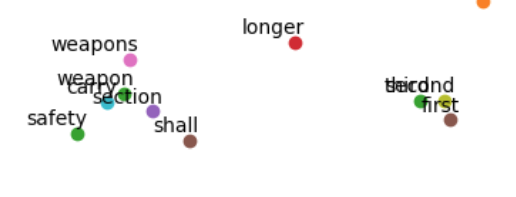
\includegraphics[width=5cm,height=2cm]{files/M128smallnews/4.png}%
		\label{fig:left}%
	} 
	\subfloat[]{%
		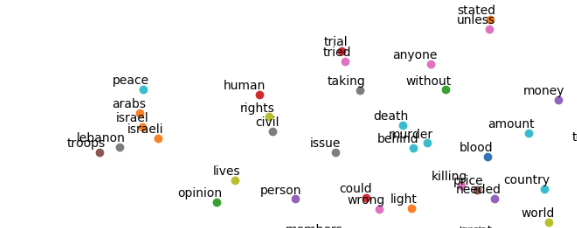
\includegraphics[width=5cm,height=2cm]{files/M128smallnews/2.png}%
		\label{fig:middle}%
	}
	\caption{Clusters of from figure, \ref{fig:t1sne}}
	\label{fig:focusOfkpcaSm}
\end{figure}
 \begin{figure}
  	\centering
  	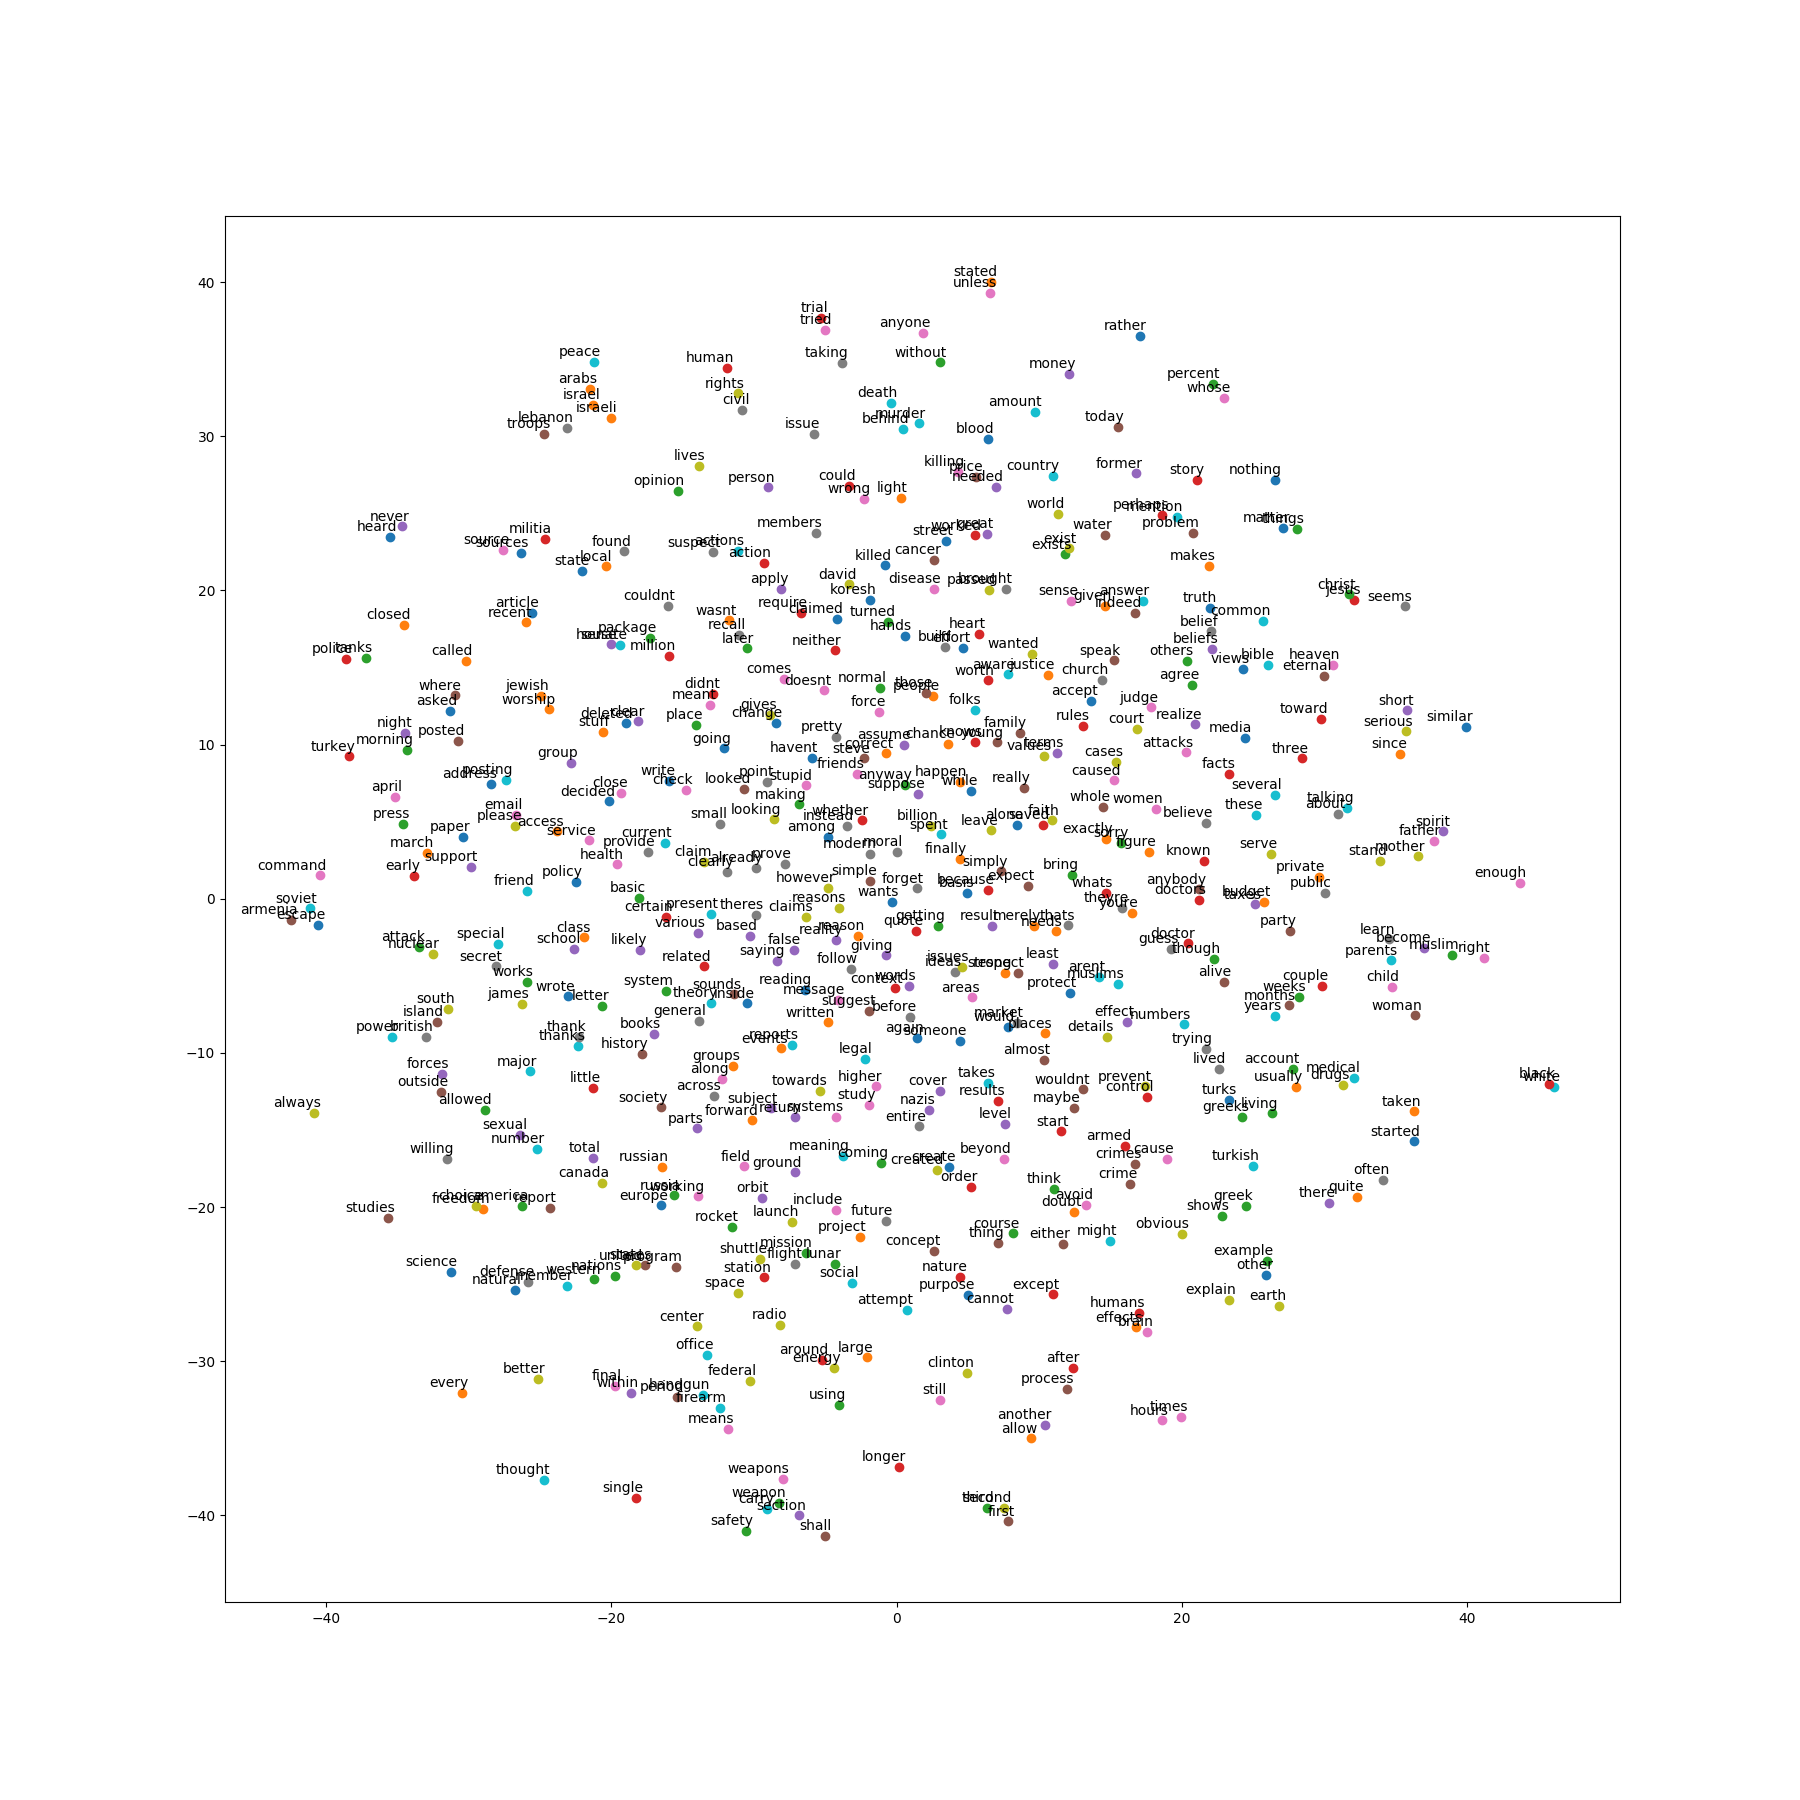
\includegraphics[width=18cm,height=15cm,keepaspectratio]{files/M128smallnews/M128smallnews.png}
  	\caption{t-SNE for KPCA skip gram model embeddings trained on vocabulary size of 20,000 words in 40,000 iteration on 20News dataset of size 350,000 words }
  	\label{fig:t1sne}
  \end{figure}
We also analyze the word embeddings using \texttt{k-nearest neighbors} of the words. These results in tables \ref{table:11} and \ref{table:13}, show that our model learns not only words with morphological similarity but also words with non-morphological similarity \textit{very quickly}.\\
In the table, \ref{table:11}, when we analyze the nearest neighbor of the word \texttt{"christ"}, at \texttt{step 0}, neighbors like \texttt{chris, christs} make sense. In the next iteration the model will start learning the semantically similar words also. At the \texttt{step 100,000} we have both semantic and morphological similar words as the nearest neighbors, \texttt{christs, savior, sinless, messiah}. Hence, initializing the model with KPCA embeddings helps the network to move towards the better neighbors "very fast".\\
 \begin{table}
 	\centering
\begin{tabular}{|l|l|l|}
	\hline
	\multicolumn{3}{|c|}{Skip gram Model with K-PCA Embeddings} \\
	\hline
	Step Number & Words & K=8 Nearest Neighbors of the word \\ \hline
	\multirow{2}{*}{Step 0} & \textbf{syria:} & wrong, wasps, hislop, falsely, randy, deacons, weary, japan \\
	& \textbf{christ:} & wrist, chris, christs, plink, sauna, opinons, cedar, mizrahi \\
	\hline
	\multirow{2}{*}{Step 20,000} & \textbf{syria:} & govt, syrian, basil, lumped, syrians, retain, holder, grossly \\
	& \textbf{christ:} & messiah, grace, lord, master, paul, christs, sins, savior \\
	 \hline
	\multirow{2}{*}{Step 40,000} & \textbf{syria:} & syrian, govt, jordan, israels, retain, syrians, dilemma, condone \\
	& \textbf{christ:} & christs, grace, messiah, savior, blessed, sins, praise, honor \\
	\hline
	\multirow{2}{*}{Step 80,000} & \textbf{syria:} & syrian, retain, jordan, israels, lebanon, sortees, sharp, govt \\
	& \textbf{christ:} & shalt, hast, christs, nutcase, savior, messiah, atoned, praise \\
	\hline
	\multirow{2}{*}{Step 100,000} & \textbf{syria:} &  syrian, retain, jordan, flows, sortees, lebanon, algeria, galilee\\
	& \textbf{christ:} & christs, shalt, savior, sinless, messiah, atoned, hast, nutcase\\
	\hline
\end{tabular}
\caption{The \textit{k}=8-nearest neighbors are generated for vectors of \textbf{128 dimension} on a vocabulary size of 20,000 words and dataset, \textbf{20NewsGroup} of size\textbf{350,000 words}}\label{table:11}
 \end{table}
%%TO DO longtable can be used 
We can also evaluate the vectors of different dimensions, \texttt{128 and 300} from tables \ref{table:11} and \ref{table:12}. Again the models are trained on same dataset and vocabulary. The vectors of dimension \texttt{300} are a bit better than those of \texttt{128}.
\begin{table}
	\centering
	\begin{tabular}{|l|l|l|}
	\hline
	\multicolumn{3}{|c|}{KPCA Skip gram Embeddings} \\
	\hline
	Step Number & Words & K=8 Nearest Neighbors of the word \\ \hline
	\multirow{2}{*}{Step 0} & \textbf{syria:} & syriac, myriad, syrias, myriads, syrian, tyrian, adrian, miriam \\
	& \textbf{christ:} & wrist, purist, christs, wrists, christi, purists, hristos, chris \\ 
	\hline
	\multirow{2}{*}{Step 20,000} & \textbf{syria:} & syrians, govt, syrian, jordan, itifada, soil, retain, viewed \\
	& \textbf{christ:} & lord, christs, depth, messiah, lucifer, gentile, bruise, creator \\
	\hline
	\multirow{2}{*}{Step 40,000} & \textbf{syria:} & syrian, jordan, retain, bombard, syrians, govt, sharp, itifada \\
	& \textbf{christ:} & messiah, honor, risen, savior, christs, sins, gentile, praying \\
	\hline
	\multirow{2}{*}{Step 80,000} & \textbf{syria:} & syrian, retain, jordan, lebanon, syrians, egypt, eldery, bombard \\
	& \textbf{christ:} & christs, savior, atoned, messiah, nutcase, velasco, againso, abraham \\
	\hline
	\multirow{2}{*}{Step 100,000} & \textbf{syria:} &  syrian, syrians, jordan, flows, sortees, lebanon, algeria, galilee\\
	& \textbf{christ:} & christs, messiah, savior, atoned, nutcase, againso, abraham, angel \\
	\hline
\end{tabular}
\caption{The \textit{k}=8-nearest neighbors are generated for vectors of \textbf{300 dimension} on a dataset, \textbf{20NewsGroup} of size, \textbf{350,000 words}}\label{table:12}
\end{table}
We can also evaluate the effect of data-set size from tables \ref{table:12} and \ref{table:13}. We can see that when trained on a larger dataset, our model tends to move more towards semantic similar vectors of the given word. It is also important to analyze that initializing the vectors with morphological similarity has given a huge boost to this move as in only 100,000 steps we have very nice semantic similar vectors which is not the case otherwise.
\begin{table}
	\centering
	\begin{tabular}{|l|l|l|}
		\hline
		\multicolumn{3}{|c|}{KPCA Skip gram Embeddings} \\
		\hline
		Step Number & Words & K=8 Nearest Neighbors of the word \\ \hline
		\multirow{2}{*}{Step 0} &\textbf{syria:} &syriac, myriad, syrias, myriads, syrian, tyrian, adrian, miriam\\
		& \textbf{christ:} &wrist, purist, christs, wrists, christi, purists, hristos, chris\\ 
		\hline
		\multirow{2}{*}{Step 20,000} & \textbf{syria:} &wily, dizzy, doorway, mayne, bald, keypad, subdued, frozen\\
		& \textbf{christ:} &burial, puts, rumors, heir, messiah, angel, truths, freely\\
		\hline
		\multirow{2}{*}{Step 40,000} & \textbf{syria:} &punjab, ciudad, sinai, libya, volga, spruce, surrey, aaai\\
		& \textbf{christ:} &lord, jesus, saints, birth, spirit, coptic, messiah, faith\\
		\hline
		\multirow{2}{*}{Step 80,000} & \textbf{syria:} &lebanon, serbia, annexed, latvia, jordan, peru, persia, turkey\\
		& \textbf{christ:} &saints, messiah, prophet, faith, mary, spirit, prayer, grail\\
		\hline
		\multirow{2}{*}{Step 100,000} & \textbf{syria:} &persia, israel, turkey, ukraine ,egypt, peru, lebanon, turkey\\
		& \textbf{christ:} &saints, messiah, prophet, baptism, mary, jesus, christian, spirit\\
		\hline
	\end{tabular}
	\caption{The \textit{k}=8-nearest neighbors are generated for vectors of \textbf{300 dimension} on a vocabulary size of 20,000 words and dataset, \textbf{Text8} of size,\textbf{17 million words}}\label{table:13}
\end{table}
When we evaluate our model word embeddings, trained for a morphological Language, \textbf{German}, we analyze that our model performs better than what it did for non-morphological language, \textbf{English}. Since most of the words which are morphologically similar, are also semantically similar, we can generate very similar neighbors in very few steps of training, as can be seen in table \ref{table:14}.
\begin{table}
	\hskip-1.5cm
	\begin{tabular}{|l|l|l|}
		\hline
		\multicolumn{3}{|c|}{KPCA Skip gram Embeddings} \\
		\hline
		Step Number & Words & K=8 Nearest Neighbors of the word \\ \hline
		\multirow{2}{*}{Step 0}
		& \textbf{macht:} &mitmacht, ohnmacht, aufmacht, ausmacht, machtlos, gemacht, lacht, gecoacht\\
		& \textbf{kinder:} &kinder-, rinder, inder, minder, binder, finder, linder, zylinder\\ 
		\hline
		\multirow{2}{*}{Step 20,000} 
		& \textbf{macht:} &aufmacht, achtung, gelacht, ansinnen, tatnacht, indische, nacht-, tafel\\
		& \textbf{kinder:} &eltern, familien, nachts, festtage, festem, festival, fests, festwirt\\ 
		\hline
		\multirow{2}{*}{Step 40,000} 
		& \textbf{macht:} &lacht, vielmehr, mache, anmelden, alltag, sorge, allemal, denke\\
		& \textbf{kinder:} &kindern, eltern, familien, lernen, gruppen, schule, betreut, lehrer\\ 
		\hline
		\multirow{2}{*}{Step 80,000} 
		& \textbf{macht:} &machte, mache, sorge, gemacht, versuche, sache, ehrgeiz, freude\\
		& \textbf{kinder:} &kindern, schueler, gruppen, lehrer, lernen, freunde, klassen, betreut\\ 
		\hline
		\multirow{2}{*}{Step 100,000} 
		& \textbf{macht:} &mache, machte, gemacht, hoert, sache, ehrgeiz, raeumt, merke\\
		& \textbf{kinder:}&kindern, gruppen, schueler, freunde, umgebung, lehrern, buechern, vereine\\ 
		\hline
	\end{tabular}
	\caption{The \textit{k}=8-nearest neighbors are generated for vectors of \textbf{300} dimension on a vocabulary size of 20000 words and subset of dataset, \textbf{news.2013.de}, of size, \textbf{52 million words}}\label{table:14}
\end{table}
We also evaluated the effect of increasing the vocabulary size as discussed in the section \ref{oov}. In table \ref{table:15}, we see that increasing the vocabulary size does not have a very major effect on the \textit{k}-nearest neighbors.
\begin{table}[H]
\begin{tabular}[htbp]{|l|l|l|l|}	
	\hline
	\multicolumn{4}{|c|}{\textbf{Comparing word2vec KPCA Embeddings with V=20,000 and V=118,000}} \\
	\hline
	\multirow{2}{*}{Step 100000}& \textbf{syria:}& sicily, ukraine, serbia, sudan& ukraine, persia, sudan, libya\\
	& \textbf{website:}& forum, site, archive, wiki &forum, site, archive, info, portal\\
	\hline
\end{tabular}
\caption{The \textit{k}=4-nearest neighbors are generated for vectors of \textbf{300} dimension on a vocabulary size of 20,000 words and vocabulary size of 118,000 words, on the dataset, \textbf{Text8}}
\label{table:15}
\end{table}
